%!TEX root = ../../main.tex
\section{Extending RADDOSE-3D for SAXS}
\label{sec:Extending RADDOSE-3D for SAXS}
To perform comparative analysis of the extent of radiation damage in SAXS experiments it is necessary to calculate the dose absorbed by the sample.
Currently dose estimates in SAXS are calculated using
\begin{equation}
    D = \f{tfE(1-T)}{V\rho},
\end{equation}
where $D$ is the dose, $t$ is the exposure time, $f$ is the X-ray flux, $E$ is the energy of the incident photons, $T$ is the transmission factor, $V$ is the illuminated volume and $\rho$ is the mass density of the sample \cite{meisburger2013breaking,jeffries2015limiting}.
To simplify the calculation of the dose, the explicit geometry of the sample is not taken into account.
A more accurate calculation can be performed if the SAXS experiment is simulated in three dimensions, providing a spatially resolved dose field.
This dose field can then be interpreted with the various dose metrics already developed for MX \cite{zeldin2013dwd,zeldin2012}.

This section presents the extensions written into RADDOSE-3D to perform simulations of SAXS experiments for improved dose calculations.

\subsection{RADDOSE-3D architecture}
\label{sub:RADDOSE-3D Architecture}
At its core, RADDOSE-3D takes a description of a crystal and exposes it to a computational beam model via a user specified exposure strategy (wedge) \cite{zeldin2013}.
The crystal is computationally modelled as a 3D voxel grid, where each grid element stores information about $x, y, z$ coordinates, the dose and the fluence.
The dose is calculated using the beam intensity at the leading edge of the voxel and the proportion of the beam that is absorbed by the voxel, which is governed by the absorption coefficient.
The beam is described by the intensity profile, photon energy and the total flux.
Finally, the wedge specifies the total angular rotation of the sample, exposure time and any rotation offsets or translations.
The structure of the program is illustrated in Figure~\ref{fig:RADDOSE-3D Flow diagram}.
A single RADDOSE-3D job performs the MX simulation on a single crystal, but it can be exposed to multiple beams with multiple wedges.
Output files giving information about the crystal state are updated after the crystal is exposed to a beam via a single wedge.
\begin{figure}
    \centering
    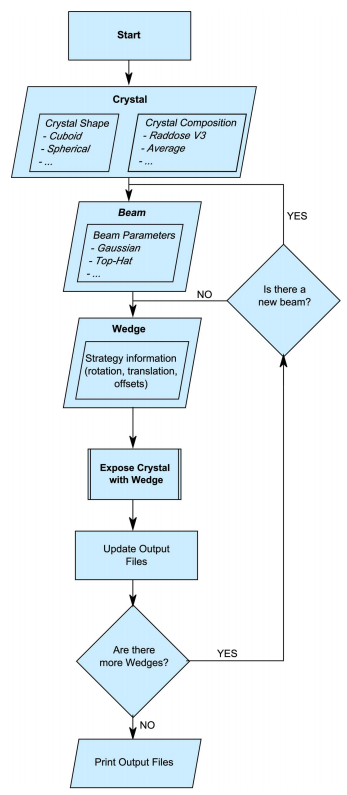
\includegraphics[width=0.6\textwidth]{figures/saxs/raddose_flow.png}
    \caption[Flow diagram illustrating the structure of the RADDOSE-3D code.]{Flow chart illustrating the structure of the RADDOSE-3D code.
    Reproduced from \cite{zeldin2013}.}
    \label{fig:RADDOSE-3D Flow diagram}
\end{figure}

At an abstract level, the crystal is defined by several properties that are typically associated with crystals in MX.
These include the unit cell volume and the number of molecules in the unit cell.
RADDOSE-3D uses this information to determine the composition of the crystal so that an absorption coefficient can be calculated.
However, there is no reason that the composition has to be defined by information specific to the crystal, in which case it is more appropriate to refer to what has been termed the ``crystal'' so far as the ``sample''.
If the sample is a liquid, as is the case in SAXS experiments, then the sample composition should be determined with different inputs.
The modular design of RADDOSE-3D enables this type of extension into be easily incorporated to the existing functionality.

\subsection{Cylindrical sample geometry}
\label{sub:Cylindrical sample geometry}
In a typical SAXS experiment, liquid samples are generally contained in, or flowed through, a cylindrical capillary during the X-ray exposure.
Therefore it is necessary for RADDOSE-3D to be able to model cylindrical sample shapes.
RADDOSE-3D had already been extended to handle polygonal shapes \cite{bury2015radiation}, which meant that it was already capable of modelling cylindrical shapes, since any 3D shape can be modelled by a series of polygons,
However, the implementation for polyhedral crystals requires the user to define the sample geometry in a non-user friendly manner.
A file specifying the geometry of the shape using a set of vertex positions, and their connectivity is required.
This is much more complex than defining the diameter of the circular cross section and the length/height of a cylinder.
Therefore a module was written that accepts a diameter and height as input and converts this into a polyhedral description (a set of vertices and faces) of a cylinder within RADDOSE-3D.
\begin{figure}
    \centering
    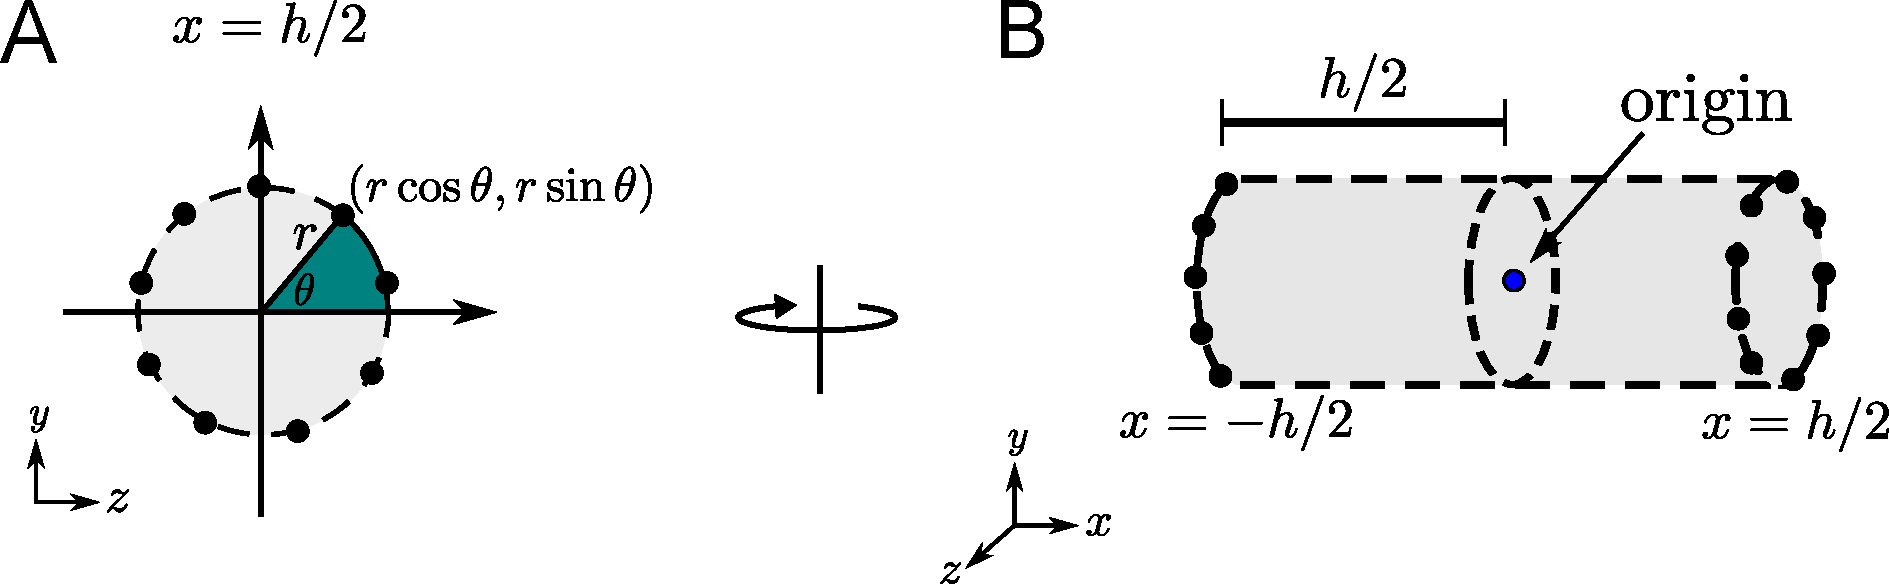
\includegraphics[width=1\textwidth]{figures/saxs/cylinder_implementation.pdf}
    \caption[Implementation of the cylindrical sample geometry in RADDOSE-3D.]{Implementation of the cylindrical sample geometry in RADDOSE-3D given user defined diameter, $d$, and height, $h$. (A) evenly spaced points around a circle are generated given the radius $r = d/2$ of the circular cross-section. RADDOSE-3D defaults to 32 points. (B) In three dimensions the points represent the circles at each end of the cylinder at a distance of $h/2$ from the origin located at the centre of the cylinder. The connectivity of these vertices is hard-coded into the RADDOSE-3D source code.}
    \label{fig:Cylindrical implementation}
\end{figure}

The cylindrical implementation, which specifies the geometry of the sample alone, not the capillary in which it is contained, is graphically depicted in Figure~\ref{fig:Cylindrical implementation} (the effect of the capillary is dealt with separately in section \ref{sub:Attenuation of X-ray flux due to capillary}).
First the points around a circle are generated using the user defined diameter of the circular cross section.
RADDOSE-3D uses 32 points around the circle by default, no matter what dimensions are specified.
The points are evenly spaced around the circle with $y, z$ coordinates $(r \cos \theta, r \sin \theta)$.
The angle (in radians) between any two consecutive points is $2 \pi / 32$.
A cylinder can be defined by the circles at either end of the shape so this is done using the final coordinate $x$.
Depending on which end a particular point is, it will have coordinates $(x, y, z) = (-h/2, r \cos \theta, r \sin \theta)$ or $(x, y, z) = (h/2, r \cos \theta, r \sin \theta)$.
Note that this assumes the origin of the system is located at the centre of the cylinder.

Regardless of the dimensions of the cylinder, the connectivity of the vertices remains the same because the number of vertices and their orientation with respect to one another is constant.
Therefore the connectivity has been hard-coded into RADDOSE-3D.
It will only ever need to be changed if the number of points is altered.
However, this parameter is not exposed to the user and hence it would only change if a developer modified the source code.

The geometry defined to create the cylinder is rotated $90^{\circ}$ about the $y$-axis compared to the usual RADDOSE-3D simulation geometry.
This means that the beam would irradiate the sample along the $x$-axis (or directly into the page looking at Figure~\ref{fig:Cylindrical implementation} A).
In a typical SAXS experiment the beam direction is along the $z$-axis defined in Figure~\ref{fig:Cylindrical implementation}  (i.e. perpendicular to the axial dimension of the cylinder).
So whenever a user specifies a SAXS experiment in RADDOSE-3D, the sample is rotated by an additional $90^{\circ}$ on the angle which the user specifies as the initial orientation of the sample to the beam (the sample geometry does not have to be specified as cylindrical).

\subsection{Determining the sample composition}
\label{sub:Determining the sample composition}
Knowledge of the atomic composition of the sample is necessary to be able to calculate the dose absorbed upon X-ray irradiation.
This is because the overall absorption coefficient of the sample, $\mu_{\text{abs}}$, is calculated from the individual atomic absorption coefficients, $\sigma_j$ as
\begin{equation}
    \mu_{\text{abs}} = (1/V_c) \sum_{j=1}^N \sigma_j,
    \label{eq:Absorption coefficient calculation}
\end{equation}
where, $V_c$ is the volume of the unit cell, $N$ is the number of atoms in the unit cell and $\sigma_j = \sigma_j^{\text{Thompson}} + \sigma_j^{\text{Compton}} + \sigma_j^{\text{Photoelectric}}$ \cite{murray2004}.
(The previous RADDOSE versions assumed $\mu_{\text{abs}} = \mu_{\text{att}}$ so equation 1 in Murray \textit{et al.} (2004) \nocite{murray2004}, which is analogous to equation \ref{eq:Absorption coefficient calculation} here, writes `$\mu_{\text{att}}$' instead of `$\mu_{\text{abs}}$').
In MX the crystal composition is calculated from the contents of the unit cell.
In SAXS the samples are liquids as opposed to crystals, and hence the notion of a unit cell does not apply.
Thus instead, the approach to determine the atomic composition of the sample is to define a volume of liquid and estimate the contents given its protein concentration and buffer composition.

First the molarity of the solution is calculated using the formula
\begin{equation}
    \text{Molarity (moles/litre)} = \f{\text{sample concentration (grams/litre)}}{\text{molecular mass (grams/mole)}}.
    \label{eq:molarity calculation}
\end{equation}
The sample concentration is provided by the user in units of grams per litre ($\equiv$ mg/ml).
The molecular mass of the molecule is calculated from other parameters provided in the user input.
If the sequence file is given for the protein (the sample can also contain DNA and RNA) then the molecular mass can be determined accurately by summing the molecular mass of each residue in the file.
Otherwise an average molecular weight is used for each residue (110 Da for protein residues, 339.5 Da for RNA residues and 327 Da for DNA residues) and the user has to specify the type and number of residues for the sample.

Secondly, a suitable volume needs to be specified to calculate the atomic composition.
A suitable volume is one that is large enough to contain at least one complete molecule.
By default this volume is defined to be (1000$\,$\AA)$^\text{3}$ but this can be changed by specifying the length, width and height dimensions of the volume in the input file using the \textit{unit cell} input keyword.

The number of monomers/molecules in the volume can now be calculated by multiplying the molarity, volume (converted to litres) and Avogadro's number ($N_A$ = 6.022 $\times$ 10$^{\text{23}}$ mol$^{\text{-1}}$), which is then rounded to the nearest integer.
The absorption coefficient can then be computed in the usual way as is described in Paithankar \textit{et al.} (2009)\nocite{pait2009}.
If there is less than 1 molecule in the volume then this is flagged up and the user is advised to increase the volume.

\subsection{Attenuation of X-ray flux due to capillary}
\label{sub:Attenuation of X-ray flux due to capillary}
In a typical MX experiment, a crystal is exposed directly to the X-ray beam.
In contrast, samples from SAXS experiments are held inside a quartz capillary.
This means that the attenuation of the X-ray flux due to the capillary needs to be taken into account before calculating the dose absorbed by the sample.

The transmission fraction of an X-ray beam due to a material with mass thickness $x$ and density $\rho$ is given by
\begin{equation}
    I/I_0 = \exp \left[ -(\mu/\rho)x\right],
    \label{eq:capillary transmission fraction}
\end{equation}
where $I$ is the emergent intensity of the beam after penetrating the material, $I_0$ is the incident intensity and $\mu/\rho$ is defined as the mass attenuation coefficient \cite{hubbell1995tables}.
The mass thickness, $x$, is defined as the mass per unit area and is given by $x = \rho t$ where $t$ is the thickness of the material.
The attenuation fraction by the capillary can hence be calculated as $1 - I/I_0$.

RADDOSE-3D requires the user to supply the thickness, density and material composition of the capillary to calculate the attenuation fraction.
The mass thickness can be directly calculated using the density and thickness as described above.
The mass attenuation coefficient is dependent on the atomic composition of the material as well as the energy of the incident photons.
The relevant values can be found online via the National Institute of Science and Technology (NIST) tables \cite{nisttable3,nisttable4}.
A section of the webpage for the mass attenuation coefficient table of carbon is shown in Figure~\ref{fig:NIST table for carbon}.
\begin{figure}
    \centering
    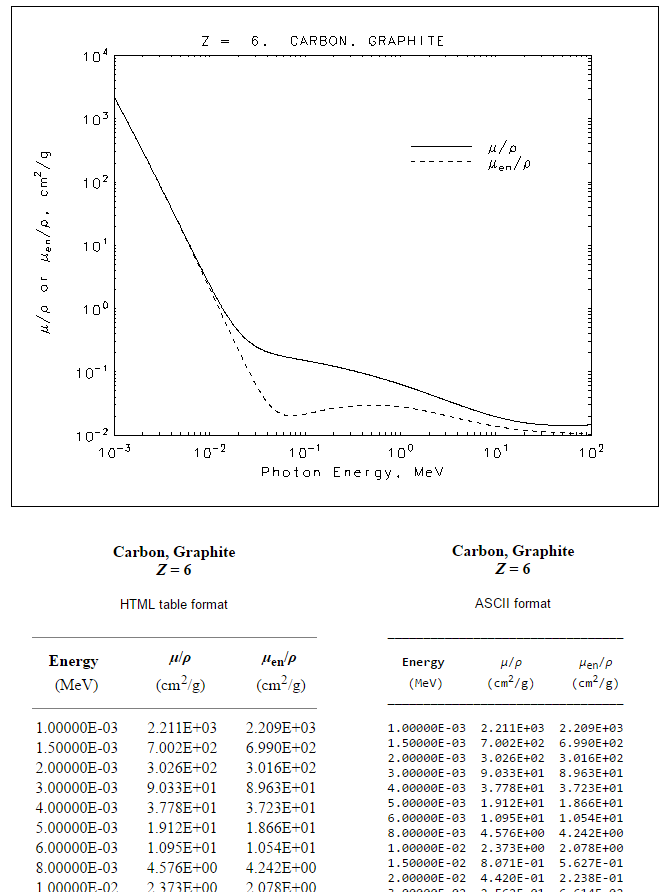
\includegraphics[width=0.7\textwidth]{figures/saxs/nist_table_carbon.png}
    \caption[X-ray mass attenuation coefficient data for carbon from NIST.]{Section of the X-ray mass attenuation coefficient data for carbon from NIST \cite{nisttable3}. The mass attenuation coefficient data are tabulated beneath the graph. The exact energy of the X-ray photons used in crystallography and SAXS (typically around 12\,keV) is not explicitly tabulated therefore the mass attenuation coefficient is obtained by linear interpolation.}
    \label{fig:NIST table for carbon}
\end{figure}
The tabulated energy values do not explicitly include the typycial energies used in crystallograpy and SAXS (around 12\,keV), so the mass attenuation coefficient is linearly interpolated between the closest values.
Mass attenuation coefficient data for various mixtures including air, borosilicate glass, water, bone and soft tissue are also tabulated in NIST table 4 \cite{nisttable4}.
These mixtures can be used directly by RADDOSE-3D.

When mixtures of atomic species are used (the most commonly used capillary material in SAXS is quartz which has elemental composition $SiO_2$) the mass attenuation coefficient is obtained using a weighted average given by
\begin{equation}
    \mu/\rho = \sum_i w_i (\mu/\rho)_i,
\end{equation}
where $w_i$ and $(\mu/\rho)_i$ are the fraction by weight and mass attenuation coefficient of the $i^{\text{th}}$ atomic constituent respectively.

\subsection{Summary of SAXS extensions}
\label{sub:Summary of SAXS extensions}
Figure~\ref{fig:Updated RADDOSE-3D Flow diagram} puts into context how the SAXS extensions fit into the RADDOSE-3D program design.
All of the changes have been made in the ``crystal'' definition which has been referred to as the \textit{sample} in this section.
\begin{figure}
    \centering
    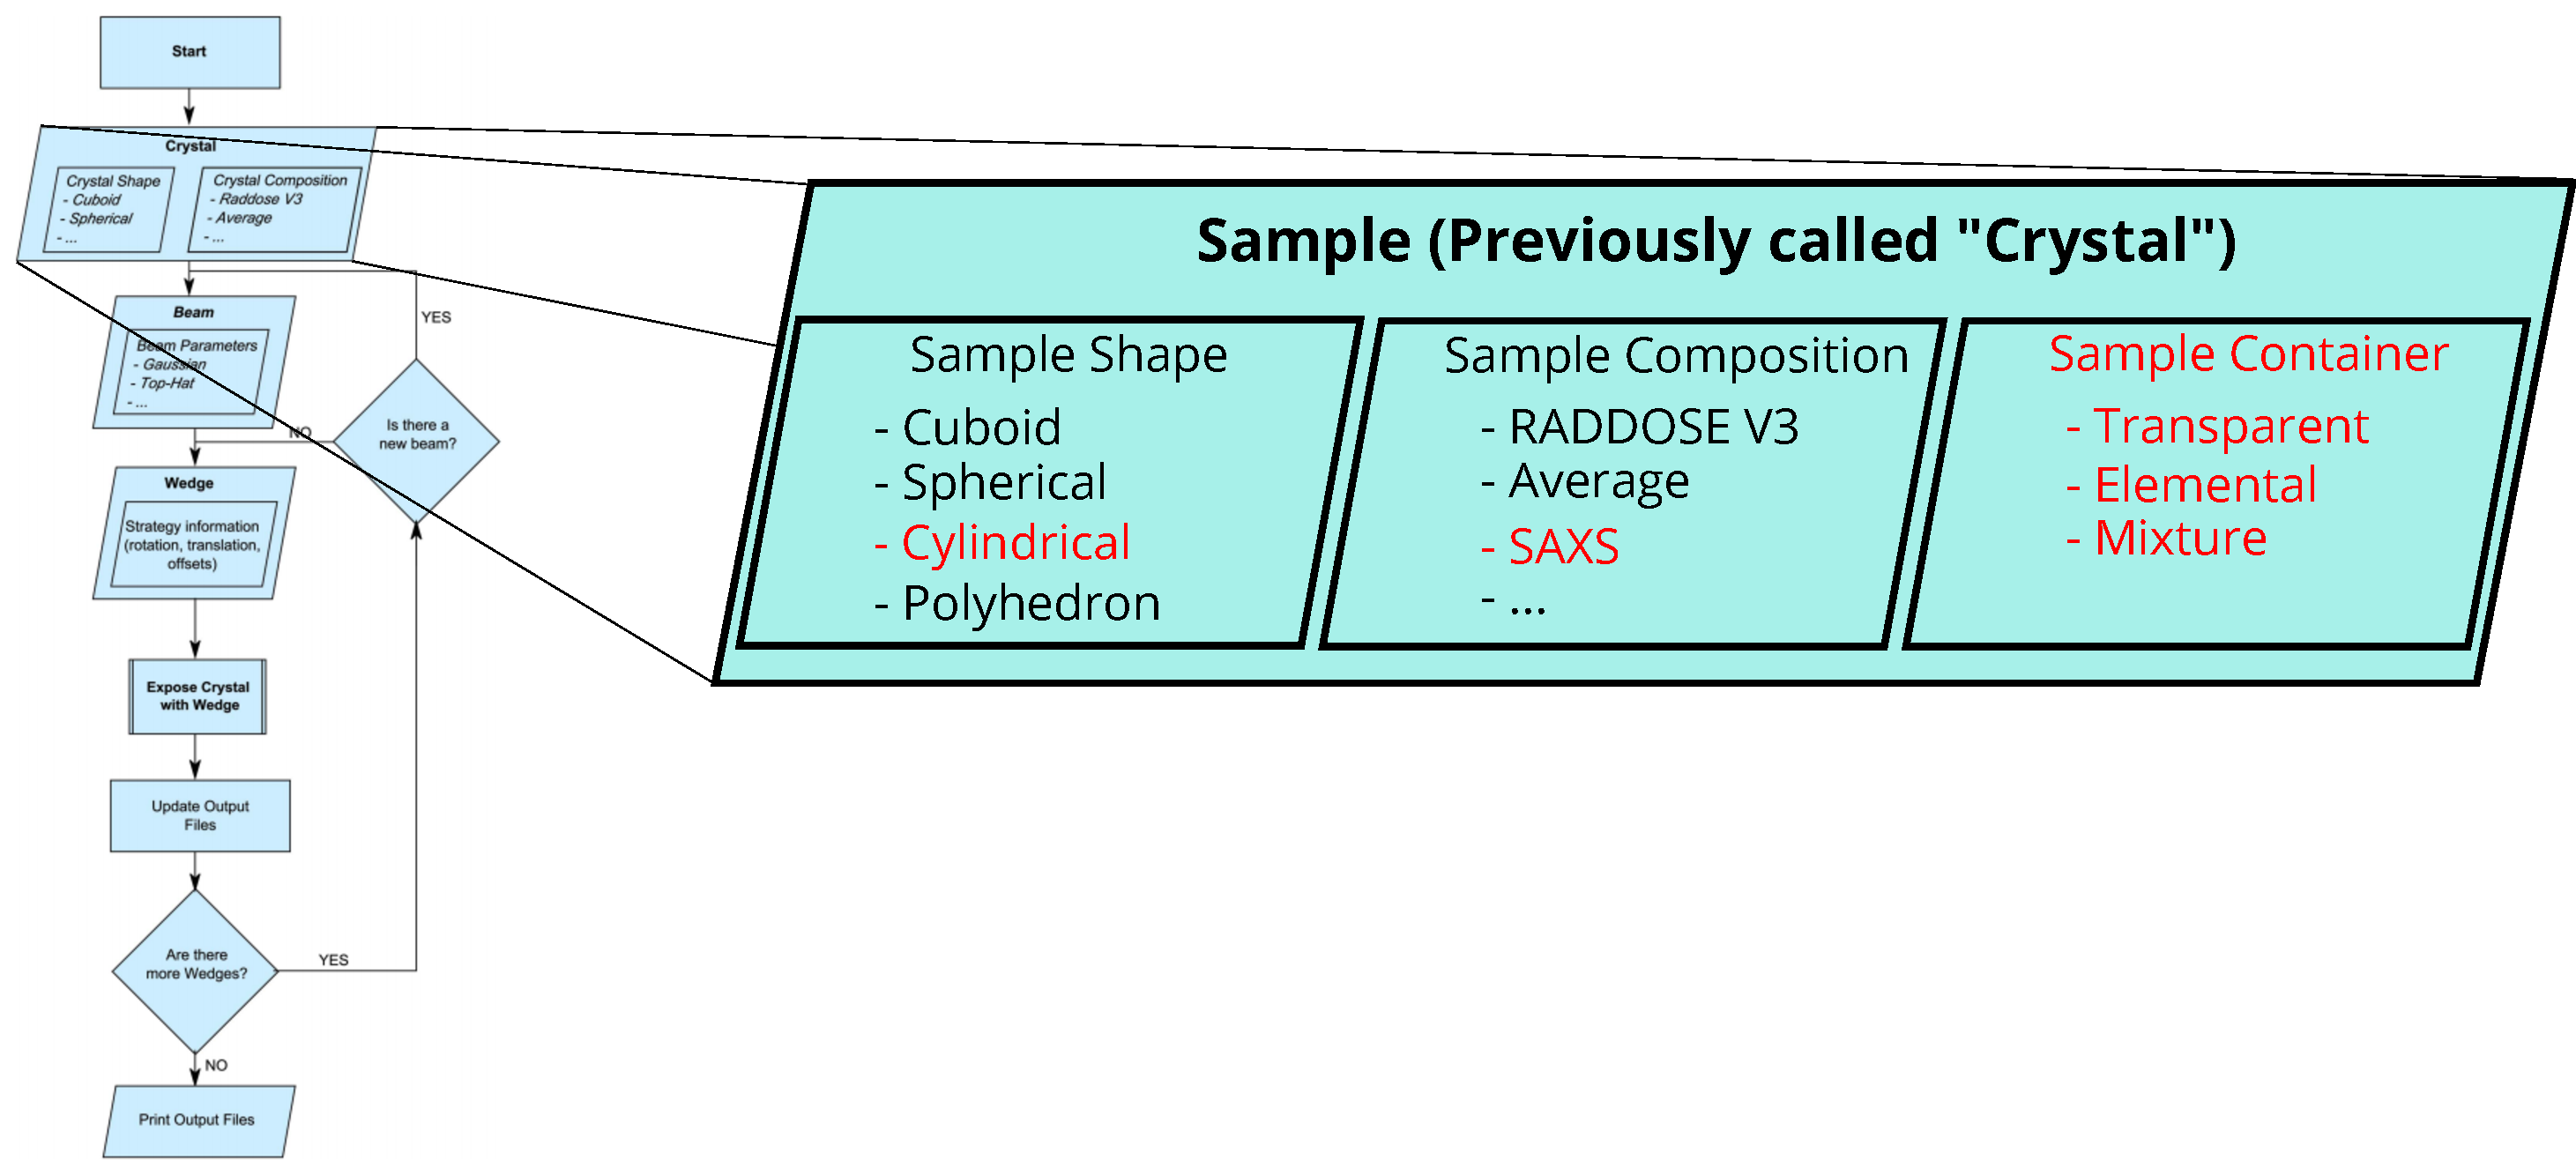
\includegraphics[width=1\textwidth]{figures/saxs/Sample_definitions.pdf}
    \caption[Updated flow diagram illustrating the structure of the RADDOSE-3D code with the SAXS extensions.]{RADDOSE-3D flowchart from Figure~\ref{fig:RADDOSE-3D Flow diagram} with the updated sample implementation, which extends the previous ``crystal'' implementation.
    The text coloured red show the SAXS extensions covered in this section.}
    \label{fig:Updated RADDOSE-3D Flow diagram}
\end{figure}

Figure~\ref{fig:SAXS Flow diagram} shows explicitly how the extensions described above combine to allow accurate dose calculations for SAXS experiments.
The cylindrical sample geometry is defined first from the specified height and diameter of the sample in the capillary.
Then the atomic sample composition is defined from the protein concentration and buffer components.
Once the container material is specified, the attenuated X-ray beam flux can then be calculated.
Finally the SAXS sample is exposed to the attenuated X-ray beam according to the `wedge' parameters.
\begin{figure}
    \centering
    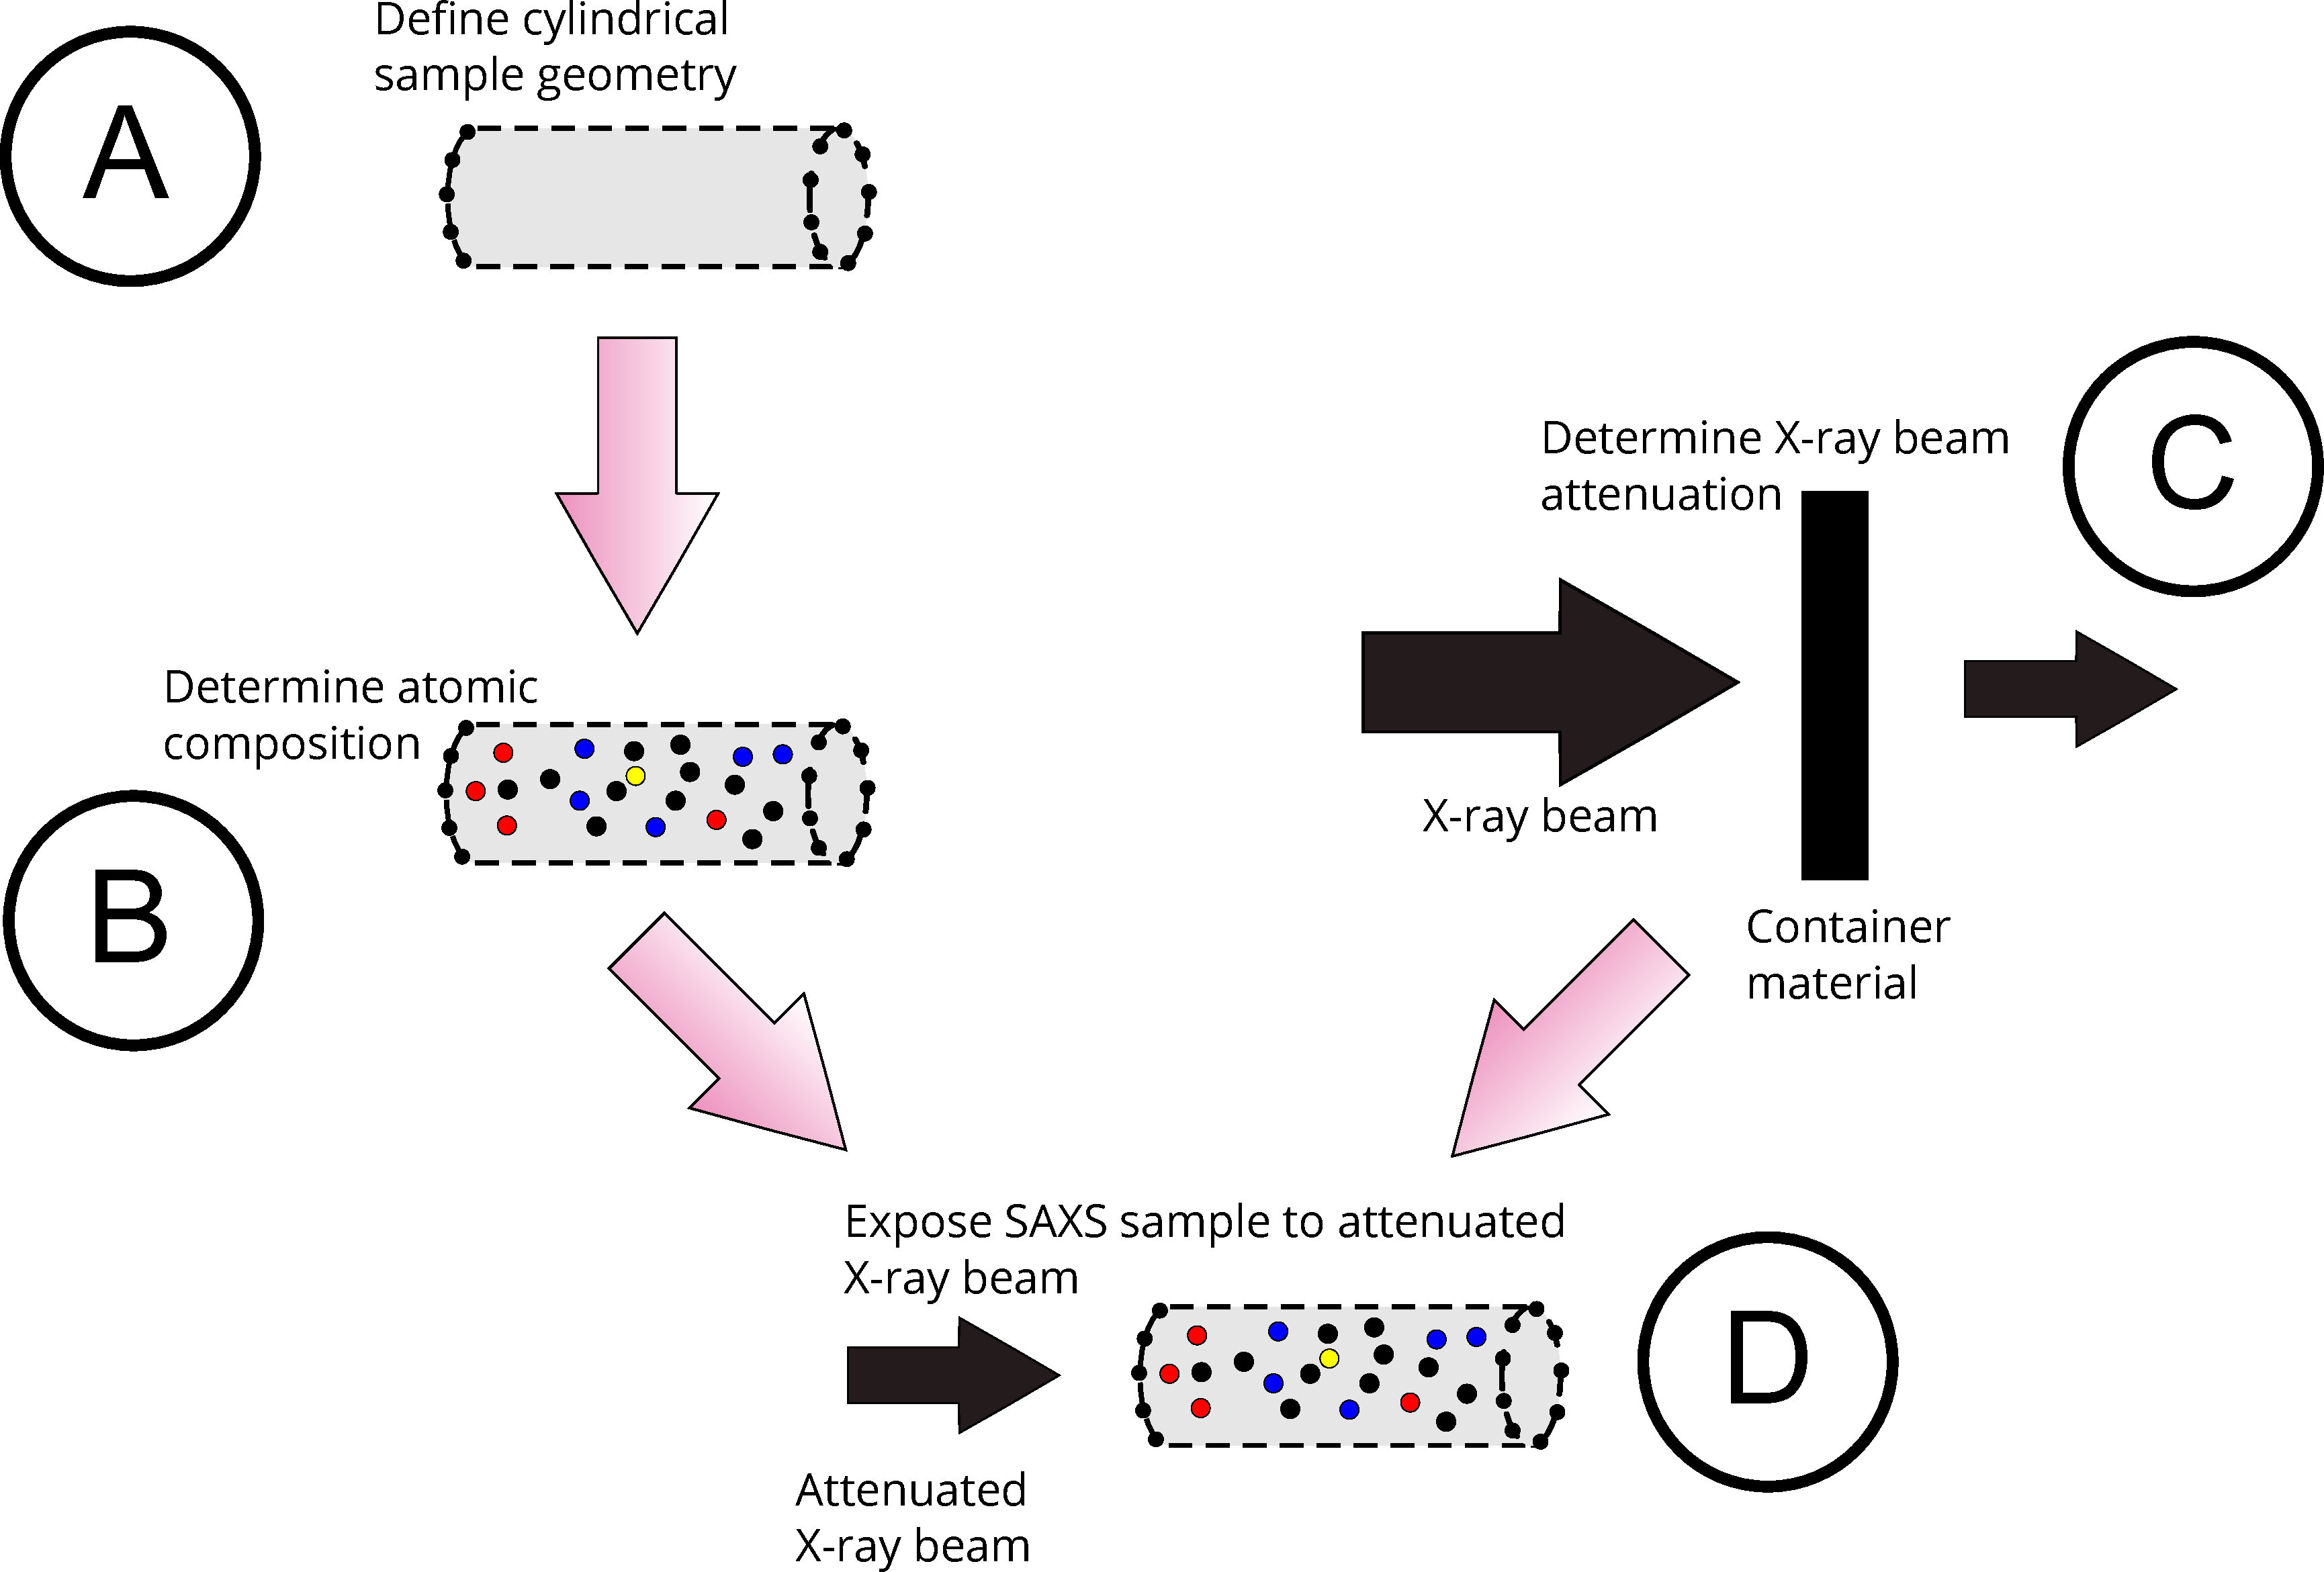
\includegraphics[width=1\textwidth]{figures/saxs/SAXS_flowchart.pdf}
    \caption[Flow diagram summarising the SAXS extensions to RADDOSE-3D.]{Flow diagram showing how the extensions described in this section are combined to enable dose calculation.
    A: Define the cylindrical geometry of the SAXS sample (section \ref{sub:Cylindrical sample geometry}).
    B: Determine the atomic composition (section \ref{sub:Determining the sample composition}).
    C: Calculate the attenuation of the beam due to the sample container (section \ref{sub:Attenuation of X-ray flux due to capillary}).
    D: Expose the SAXS sample to the attenuated beam according to the defined wedge.}
    \label{fig:SAXS Flow diagram}
\end{figure}

\subsection{Model considerations}
\label{sub:Model considerations}
The model of the SAXS experiment in RADDOSE-3D makes many implicit assumptions.
For instance, with regards to the capillary, the atomic composition is assumed to be uniform throughout, and the thickness to be constant around the entire sample volume.
The advantage of these assumptions are that the attenuation by the capillary only needs to be calculated once, regardless of any movement or rotation of the capillary.
This is valid for a cylindrical capillary since the thickness penetrated by the X-ray beam is the same regardless of any rotations or translations.

The sample itself is assumed static, moving as a rigid body when rotated or translated, and completely filling the capillary.
This greatly reduces the computational cost when compared to the possibility of modelling the exact fluid dynamics.
The assumption that the capillary volume is completely filled is generally valid since this is usually the case during an experiment.
The static assumption is not always valid, especially when the sample is flowed through the capillary.
Hopkins and Thorne calculated that for typical experimental parameters (capillary diameters: 1.5-2$\,$mm, flow velocities: 0.5-15$\,$mm$\,$s$^{\text{-1}}$) the Reynolds numbers\footnote{The Reynolds number is defined as the ratio of inertial forces to viscous forces and is a quantity used in fluid mechanics to determine properties of fluid flow \cite{purcell1977life}.} are in the range 1-25 implying a laminar flow regime \cite{hopkins2016quantifying}.
In this case the velocity profile is expected to exhibit the quadratic Poiseuille flow profile, which arises from the axial symmetry and no-slip boundary assumptions (the velocity at the centre of the tube moves the fastest while the velocity at the boundary is equal to zero provided the capillary is also stationary).
Furthermore, Hopkins and Thorne also calculated that the residence times of the sample in the beam were too short for any appreciable radial diffusive mixing, hence the flow profile results in radius-dependent residence times in the X-ray beam.
Therefore the static assumption here will give misleading dose values if calculated for experiments where the sample is flowed through the beam.

Hopkins and Thorne additionally discuss diffusive turnover as a phenomenon that will affect the dose calculation \cite{hopkins2016quantifying}.
Molecules have the ability to diffuse into and out of the illuminated volume, with the additional complexity that a non-uniform beam profile will cause differential diffusion across the beam.
In the current work, no account was taken for molecular diffusion.
Extrapolation of the plot from \cite{hopkins2016quantifying} (reproduced in Figure~\ref{fig:Diffusive turnover effect} ) shows that diffusion is likely to be negligible for the experiment performed here (section \ref{sec:Experimental methods - SAXS}) where the beam size was 600 $\times$ 600$\,\mu m^{\text{2}}$ and the total exposure time was 120 seconds.
\begin{figure}
    \centering
    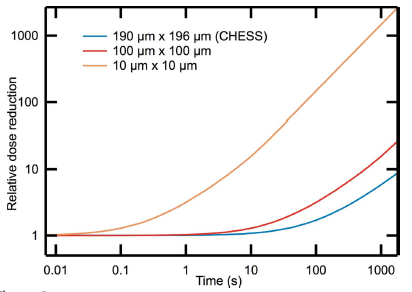
\includegraphics[width=0.75\textwidth]{figures/saxs/diffusive_turnover_effect.png}
    \caption[Effect of diffusive turnover on the dose in SAXS.]{Reduction in the dose absorbed by the sample due to diffusive exchange of lysozyme against time for three beam sizes.
    Extrapolation of these curves for a beam size of 600 $\times$ 600$\,\mu m^{\text{2}}$ along with 120 second exposure times suggests that the dose reduction due to diffusive turnover is negligible for the experiment reported in this chapter.
    Figure reproduced from \cite{hopkins2016quantifying}.}
    \label{fig:Diffusive turnover effect}
\end{figure}

The SAXS sample can also be manipulated in the same way as a crystal in RADDOSE-3D.
Hence helical scanning, translations and rotations of the sample can all be performed.
Figure~\ref{fig:SAXS cylinder rotated} is the final dose state of a glucose isomerase sample in an experiment where the sample was rotated 180$^{\circ}$ for a total of 200 seconds in a 700 $\times$ 700 $\mu m^{\text{2}}$ top-hat profile beam with a flux of 1.51 $\times$ 10$^{\text{13}}\,$ph/s and an incident photon energy of 12.1$\,$keV.
\begin{figure}
    \centering
    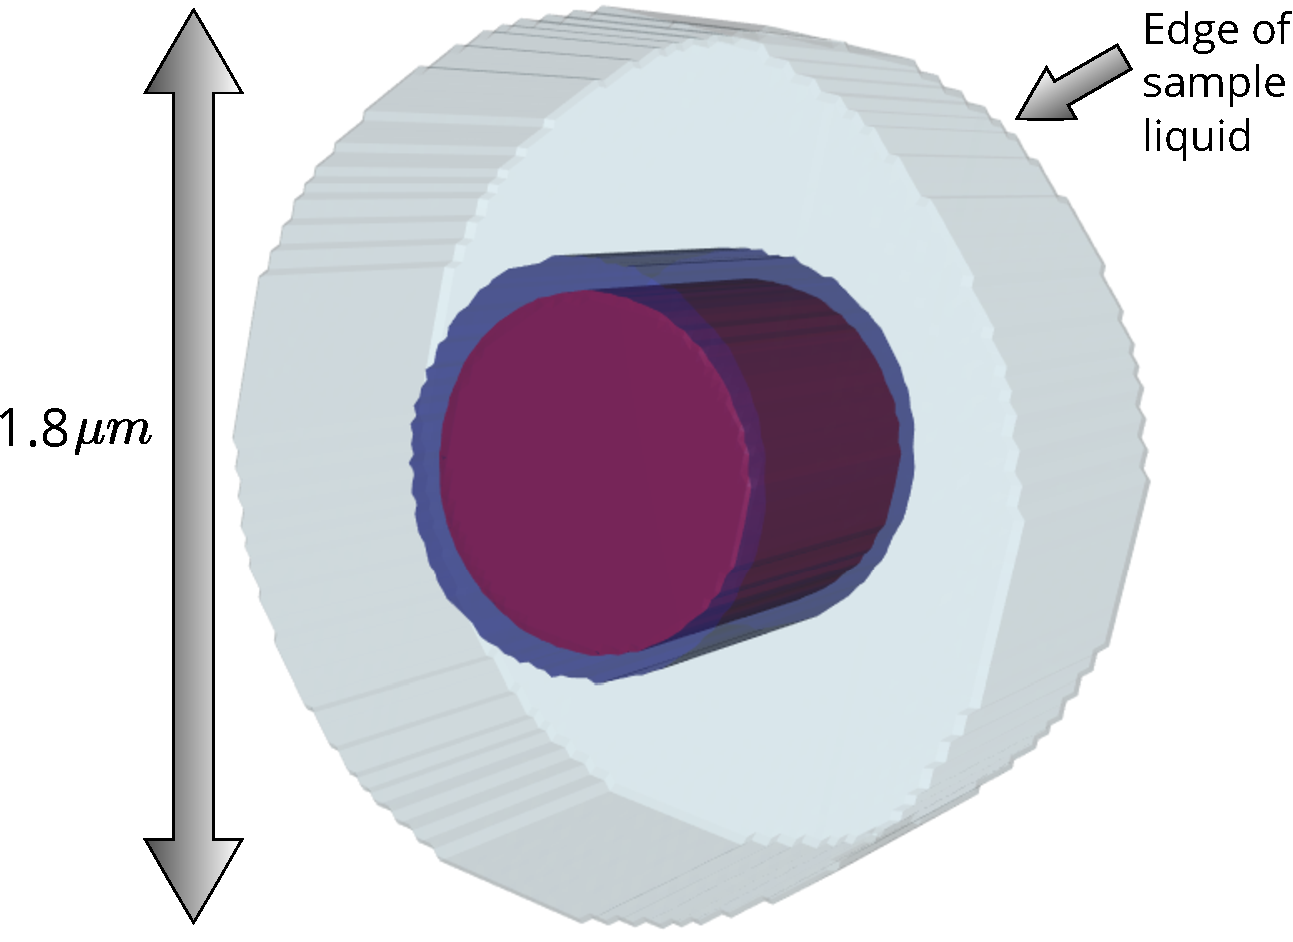
\includegraphics[width=0.75\textwidth]{figures/saxs/SAXScylinder.pdf}
    \caption[RADDOSE-3D dose contour plot of a cylindrical SAXS sample.]{Final dose state of a glucose isomerase sample in an experiment where the sample was rotated 180$^{\circ}$ in a 700\,$\mu m$ $\times$ 700\,$\mu m $ top-hat profile beam with a beam flux of 1.51 $\times$ 10$^{\text{13}}\,$ph/s and an incident energy of 12.1\,keV for a total exposure time of 200 seconds.
    The capillary was treated as completely transparent to the X-rays so there was no attenuation.
    The dose state is only calculated and shown for the sample, not the capillary.
    The contours correspond to dose iso-surfaces: light blue = 0.1\,MGy, dark blue = 1.5\,MGy and purple = 2\,MGy.}
    \label{fig:SAXS cylinder rotated}
\end{figure}
